\documentclass[11pt,letterpaper]{article}
\usepackage[utf8]{inputenc}
\usepackage[top=1in,bottom=1in,left=1in,right=1in]{geometry}
\usepackage{amsmath}
\usepackage{amsfonts}
\usepackage{amssymb}
\usepackage{amsthm}
\usepackage{bm}
\usepackage{braket}
\usepackage{cancel}
\usepackage{enumitem}
\usepackage{float}
\usepackage{graphicx}
\usepackage{hyperref}
\usepackage{mathabx}
\usepackage{parskip}
\usepackage{subcaption}
\usepackage{tensor}
\usepackage{titlesec}
\usepackage{titling}
\usepackage{listings}




% \titlelabel{(\thetitle)\quad}
\titleformat*{\section}{\large\bfseries}
\titleformat*{\subsection}{\normalsize\bfseries}
\setlength{\droptitle}{-5em}



\let\Re\relax
\DeclareMathOperator{\Re}{Re}
\let\Im\relax
\DeclareMathOperator{\Im}{Im}

\DeclareMathOperator*{\argmin}{arg\,min}
\DeclareMathOperator*{\argmax}{arg\,max}
\DeclareMathOperator*{\arginf}{arg\,inf}
\DeclareMathOperator*{\argsup}{arg\,sup}


\newcommand{\bhat}[1]{\hat{\bm{#1}}}
\newcommand{\R}{\mathbb{R}}

\renewcommand{\thesubsection}{\normalsize \alph{subsection}}
\renewcommand{\d}{\mathrm{d}}
\renewcommand{\vec}[1]{\bm{#1}}
\newcommand{\del}{\vec{\nabla}}
\newcommand{\e}{\epsilon}
\newcommand{\tpd}[3]{\left( \frac{\partial #1}{\partial #2} \right)_{#3}}
\newcommand{\pd}[2]{\frac{\partial #1}{\partial #2}}
\newcommand{\spd}[2]{\frac{\partial^2 #1}{\partial {#2}^2}}
\def\dbar{{\mathchar'26\mkern-12mu d}}

\allowdisplaybreaks


\author{Sam Kowash}
\numberwithin{equation}{section}
\numberwithin{figure}{section}
\title{CSE 546 HW \#2}

\begin{document}
\maketitle

{\bf Acknowledgments:} I collaborated on parts of this homework with Tyler Blanton, Michael Ross, and Nick Ruof.

\section{A Taste of Learning Theory}
\begin{enumerate}
	\item Let $X \in \mathbb{R}^d$ a random feature vector, and $Y \in \{1,\ldots,K\}$ a random label for $K\in \mathbb{N}$ with joint distribution $P_{XY}$. We consider a randomized classifier $\delta(x)$ which maps a value $x\in\mathbb{R}^d$ to some $y \in \{1,\ldots,K\}$ with probability $\alpha(x,y) \equiv P(\delta(x)=y)$ subject to $\sum_{y=1}^K \alpha(x,y) = 1$ for all $x$. The risk of the classifier $\delta$ is
	%
	\begin{align*}
		R(\delta) &\equiv \mathbb{E}_{XY,\delta}\left[\bm{1}\{\delta(X) \neq Y\}\right],
	\end{align*}
	%
	which we should interpret as the expected rate of misclassification. A classifier $\delta$ is called deterministic if $\alpha(x,y) \in \{0,1\}$ for all $x,y$. Further, we call a classifier $\delta_\ast$ a Bayes classifier if $\delta_\ast \in \arginf_\delta R(\delta)$.

	If we first take the expectation over outcomes of $\delta$ (by conditioning on $X$ and $Y$), we find
	%
	\begin{align*}
		R(\delta) &= \mathbb{E}_{XY}\left[1-\alpha(X,Y)\right],
	\end{align*}
	%
	since the indicator function is 1 except for the single outcome where $\delta(x)=y$, which occurs with probability $\alpha(x,y)$. It is then clear that minimizing $R(\delta)$ is equivalent to \emph{maximizing} $\mathbb{E}_{XY}[\alpha(X,Y)]$; the assignments of $\alpha(x,y)$ which do this are our Bayes optimal classifiers.

	Define $p_k(x) = \mathbb{P}(Y=k \mid X=x)$ and $\alpha_k(x) = \alpha(X,k)$. Then
	%
	\begin{align*}
		\mathbb{E}_{XY}(\alpha(X,Y)) = \mathbb{E}_X\left[\mathbb{E}_{Y\mid X} \left[\alpha(x,Y) \mid X=x\right]\right] = \mathbb{E}_X\left[\sum_{k=1}^K p_k(X) \alpha_k(X)\right]
	\end{align*}
	%
	Fixing an $x$ for a moment, note that
	%
	\begin{align*}
		\sum_{k=1}^K p_k \alpha_k \leq \sum_{k=1}^K \alpha_k \max_i \{p_i\} = \max_i \{p_i\} \sum_{k=1}^K \alpha_k = \max_i \{p_i\},
	\end{align*}
	%
	so any $\delta$ which saturates this bound for each $x$ is a Bayes classifier. This is clearly achieved by any assignment satisfying $\alpha(x,i) = 0$ for $i \notin \argmax_{k} p_k(x)$. A deterministic member of this class is the rule that always predicts the smallest $i \in \argmax_k p_k(x)$.


















	\item Suppose we grab $n$ data samples $(x_i,y_i)$ i.i.d. from $P_{XY}$ where $y_i \in \{-1,1\}$ and $x_i \in \mathcal{X}$ where $\mathcal{X}$ is some set. Let $f: \mathcal{X} \to \{-1,1\}$ be a deterministic classifier with true risk
	%
	\begin{align*}
		R(f) &= \mathbb{E}_{XY}\left[\bm{1}(f(X) \neq Y)\right].
	\end{align*}
	%
	and empirical risk
	%
	\begin{align*}
		\hat{R}_n(f) &= \frac{1}{n} \sum_{i=1}^n \bm{1}(f(x_i) \neq y_i).
	\end{align*}




	\begin{enumerate}
		\item We wish to estimate the true risk of some classifier $\tilde{f}$. The empirical risk $\hat{R}_n(\tilde{f})$ is an average of $n$ i.i.d.\ random variables---the indicator functions $\bm{1}(f(x_i) \neq y_i)$---and the true risk is the expected value of each of those random variables. This satisfies the hypotheses of Hoeffding's inequality, so for any $\e \geq 0$ we have
		%
		\begin{align*}
			\mathbb{P}\left(\left|\hat{R}_n(\tilde{f}) - R(\tilde{f})\right| \geq \e\right) &\leq 2 e^{-2n\e^2}.
		\end{align*}
		%
		We can rewrite this probability in terms of its complement, giving
		%
		\begin{align*}
			1 - \mathbb{P}\left(\left|\hat{R}_n(\tilde{f}) - R(\tilde{f})\right| < \e\right) &\leq 2e^{-2n\e^2}\\
			\mathbb{P}\left(\left|\hat{R}_n(\tilde{f}) - R(\tilde{f})\right| < \e\right) &\geq 1 - 2e^{-2n\e^2}.
		\end{align*}
		%
		Thus, with confidence $1-\delta$, the empirical risk falls within $A$ of the true loss, where
		%
		\begin{align*}
			A &= \sqrt{-\frac{\ln \delta/2}{2n}}.
		\end{align*}






		\item Let $\mathcal{F} = \{f_1,\ldots,f_k\}$ be a set of classifying rules that is devised based on a prior hypothesis about $P_{XY}$. Since the classifiers are functions of a single variable, the set of indicator variables remains independent; the distribution of the $i$th indicator is not ``tainted'' by information about any other. The hypotheses of Hoeffding's inequality are just as well satisfied by any member of $\mathcal{F}$ as they were by the arbitrary $\tilde{f}$ considered above, and the previous confidence interval holds. In particular, it holds for the best-in-class function
		%
		\begin{align*}
			f^\ast &= \argmin_{f \in \mathcal{F}} R(f).
		\end{align*}





		\item We now consider the empirical risk minimizer
		%
		\begin{align*}
			\hat{f} &= \argmin_{f \in \mathcal{F}} \hat{R}_n(f).
		\end{align*}
		%
		Although we used our data to select $\hat{f}$ from the class $\mathcal{F}$, there is still no dependence between the indicators $\bm{1}\{f(x_i)\neq y_i\}$, because the value of $f(x_i)$ does not depend on any $y_i$ or $x_{j\neq i}$ and the draws $\{(x_i,y_i)\}$ are independent of each other by hypothesis. Thus, we can proceed just as in the original case and obtain the same confidence interval on the deviation of $\hat{R}_n(\hat{f})$ from $R(\hat{f})$.




		\item I'm not sure that there is such an example with the previous assumption that $\mathcal{F}$ is finite.

		If $\mathcal{X}$ is finite, then there is nonzero probability to sample the same element twice. To achieve zero empirical risk, $P_{XY}$ must never allow us to sample the same $x$ with different $y$s. But, since there is nonzero probability to sample all of $\mathcal{X}$ for $n \geq |\mathcal{X}|$, zero empirical risk is only possible if $\mathcal{F}$ contains a function that maps every $x$ to its sole allowed $y$, but that function clearly has both zero empirical risk \emph{and} zero true risk, contradicting the problem statement.

		If $\mathcal{X}$ is countable, the double-sampling issue still demands that $P_{XY}$ uniquely determine $y$ for each $x$. We don't have to worry about sampling the entire set, but we now seem to need an infinite function class to achieve zero empirical risk. If uncountable, it seems even worse. If this is possible, I'm really curious as to how.









		\item To find a confidence interval that can be satisfied by all $f \in \mathcal{F}$ simultaneously with probability at least $1-\delta$, note that for $\e \geq 0$,
		%
		\begin{align*}
			\mathbb{P}\left[\bigcup_{i=1}^k |\hat{R}_n(f_i) - R(f_i)| \geq \e\right] &\leq \sum_{i=1}^k \mathbb{P}\left(|\hat{R}_n(f_i) - R(f_i)| \geq \e\right)
		\end{align*}
		%
		by the union bound, and applying Hoeffding's inequality to each term as justified above,
		%
		\begin{align*}
			\mathbb{P}\left[\bigcup_{i=1}^k |\hat{R}_n(f_i) - R(f_i)| \geq \e\right] &\leq \sum_{i=1}^k 2e^{-2n\e^2} = 2ke^{-2n\e^2}.
		\end{align*}
		%
		Using De Morgan's law to identify the complement of the event on the left-hand side, we rewrite just as before to get
		%
		\begin{align*}
			1 - \mathbb{P}\left[\bigcap_{i=1}^k |\hat{R}_n(f_i) - R(f_i)|<\e\right] &\leq 2k e^{-2n\e^2}\\
			\mathbb{P}\left[\bigcap_{i=1}^k |\hat{R}_n(f_i) - R(f_i)|<\e\right] &\geq 1 - 2k e^{-2n\e^2}.
		\end{align*}
		%
		From this we can see that
		%
		\begin{align*}
			\mathbb{P}\left(\text{for all $f\in\mathcal{F}$, } |\hat{R}_n(f) - R(f)| \leq B\right) &\geq 1-\delta,
		\end{align*}
		%
		where
		%
		\begin{align*}
			1 - \delta &= 1 - 2k e^{-2nB^2}\\
			\ln \frac{\delta}{2k} &= -2nB^2\\
			B &= \sqrt{-\frac{\ln \delta/(2k)}{2n}}.
		\end{align*}








		\item The confidence interval for the ERM should be exactly the same as that found in part (a), as could also be seen by considering the degenerate class of one function, which gives $k=1$ in the above result and reproduces that of part (a).







		\item Because $\hat{f}$ minimizes empirical risk and $f^\ast$ the true risk, we have
		%
		\begin{align*}
			0 &\leq R(\hat{f}) - R(f^\ast)\\
			0 &\leq \hat{R}_n(f^\ast) - \hat{R}_n(\hat{f}),
		\end{align*}
		%
		and so
		%
		\begin{align*}
			0 &\leq R(\hat{f})-R(f^\ast) \leq [\hat{R}_n(f^\ast) - R(f^\ast)] - [\hat{R}_n(\hat{f}) - R(\hat{f})].
		\end{align*}
		%
		Then also
		%
		\begin{align*}
			0 &\leq R(\hat{f})-R(f^\ast) \leq \left|\hat{R}_n(f^\ast) - R(f^\ast)\right| + \left|\hat{R}_n(\hat{f}) - R(\hat{f})\right|.
		\end{align*}
		%
		If we assume $\hat{f} \neq f^\ast$, then the previous result tells us that for any threshold $\delta$,
		%
		\begin{align*}
			\mathcal{P}\left[ \left(\left|\hat{R}_n(f^\ast) - R(f^\ast)\right| \leq B\right) \cap \left(\left|\hat{R}_n(\hat{f}) - R(\hat{f})\right| \leq B\right)\right] &\geq 1-\delta,
		\end{align*}
		%
		where
		%
		\begin{align*}
			B &= \sqrt{-\frac{\ln \delta/4}{2n}}
		\end{align*}
		%
		since we are considering a class of $k=2$ functions. Thus, we can say that with probability at least $1-\delta$,
		%
		\begin{align*}
			 \left|\hat{R}_n(f^\ast) - R(f^\ast)\right| + \left|\hat{R}_n(\hat{f}) - R(\hat{f})\right| &\leq C = 2B = 2\sqrt{-\frac{\ln \delta/4}{2n}}.
		\end{align*}












		\item Fix $f\in \mathcal{F}$ and suppose $R(f) \geq \e$. This implies that the probability for an arbitrary $(x,y)$ to be correctly classified by $f$ is no greater than $1-\e$, so the probability of correctly classifying a set of $n$ points (that is, $\mathbb{P}(\hat{R}_n(f) = 0)$) is no greater than $(1-\e)^n$. Note (recalling $0 < \e$) that if $\e<1$,
		%
		\begin{align*}
			\ln\left((1-\e)^n\right) &= n \ln(1-\e) = -n \sum_{k=1}^\infty \frac{\e^k}{k} \leq -n \e,
		\end{align*}
		%
		so that
		\begin{align*}
			(1-\e)^n &\leq e^{-n \e}.
		\end{align*}
		%
		We patch the hole in the above by noting that this relation holds if we plug in $\e =1$ as well. Thus,
		%
		\begin{align*}
			\mathbb{P}(\hat{R}_n(f) = 0) &\leq e^{-n \e}.
		\end{align*}

		Unsure how to continue this to compute regret.




		\item Regret.


	\end{enumerate}

\end{enumerate}

























\section{Programming}
\begin{enumerate}
	\setcounter{enumi}{2}
	\item 
	We generated $n=500$ points $(x_i,y_i) \in \R^d \times \R$ according to the model $y_i = w^T x_i + \e_i$, where
	%
	\begin{align*}
		w_j &= \begin{cases}
			j/k &\text{if } j \in \{1,\ldots,k\}\\
			0 & \text{otherwise}\\
		\end{cases}
	\end{align*}
	%
	and $\e_i \sim \mathcal{N}(0,\sigma^2)$ with $k=100$, $d=1000$, and $\sigma = 1$. We then computed a regularization path on this data for the parameter $\lambda$ in the lasso objective as shown in Fig.~\ref{fig:lasso_reg} and observed the false discovery and true positive rates for the relevant/irrelevant features as seen in Fig.~\ref{fig:tprfdr}. As $\lambda$ increases (to the left in Fig.~\ref{fig:lasso_reg}), fewer and fewer features are selected, and vice versa, with most features selected by $\lambda \sim 10^{-3}$. Also as $\lambda$ grows, the false discovery rate falls as features are eliminated, and the true positive rate falls to some extent with it.


	\begin{figure}[H]
		\centering
		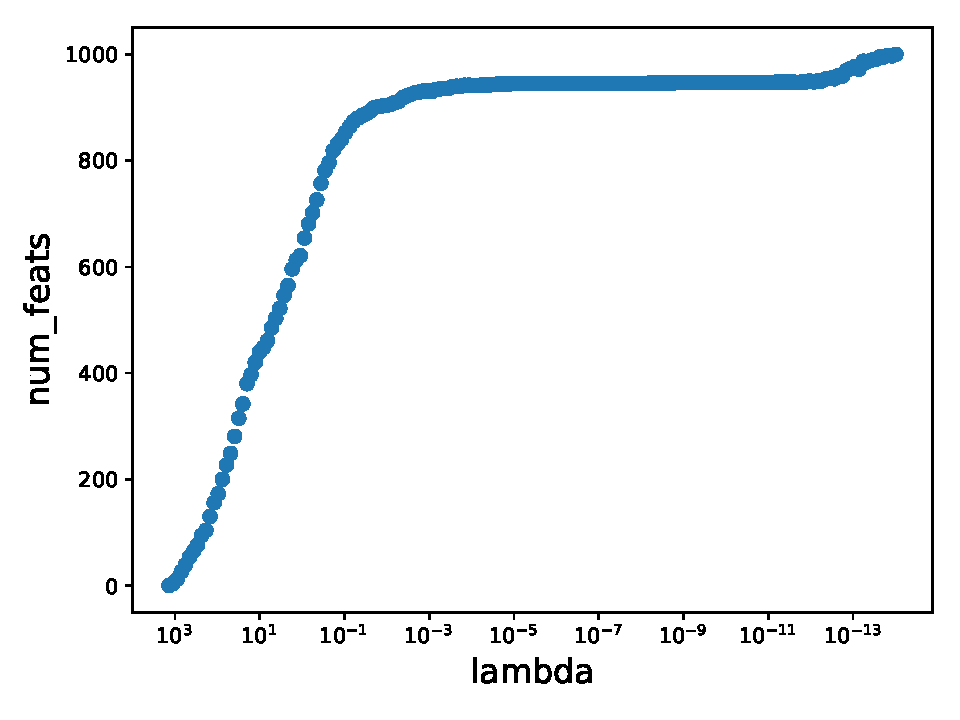
\includegraphics[width=0.6\textwidth]{figures/synth_nfeats_80.pdf}
		\caption{Number of nonzero features vs. $\lambda$ for lasso on synthetic data}
		\label{fig:lasso_reg}
	\end{figure}

	\begin{figure}[H]
		\centering
		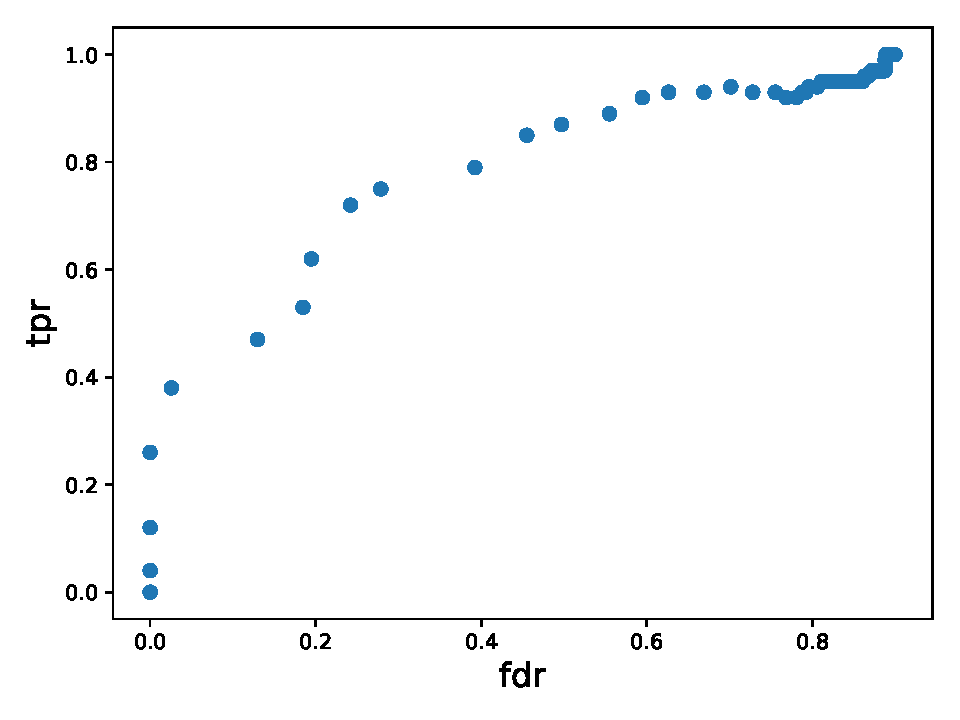
\includegraphics[width=0.6\textwidth]{figures/synth_fdr-tpr_80.pdf}
		\caption{TPR vs. FDR for lasso on synthetic data}
		\label{fig:tprfdr}
	\end{figure}











	\item
	\begin{enumerate}
		\item We next computed a regularization path on the provided Yelp data, depicted in Fig.~\ref{fig:yelp_feats}, and used a validation holdout set to assess regression performance, shown in \ref{fig:yelp_err}. We found that validation error was best around $\lambda=1.11$.

			\begin{figure}[H]
				\centering
				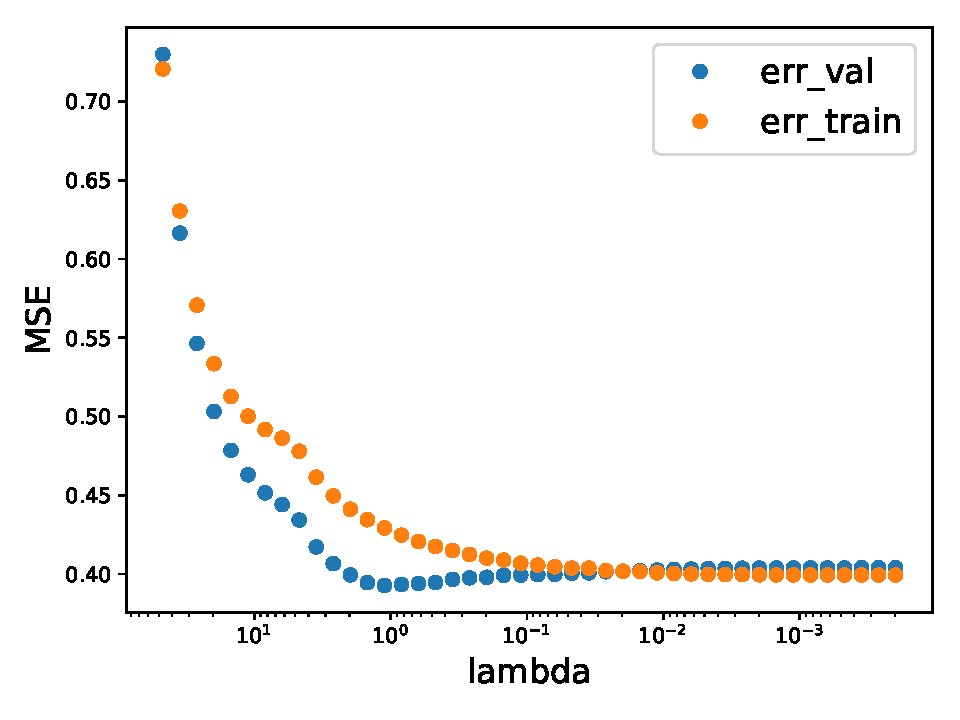
\includegraphics[width=.6\textwidth]{figures/yelp_errs.pdf}
				\caption{Validation and training error vs $\lambda$ on Yelp data}
				\label{fig:yelp_err}
			\end{figure}

			\begin{figure}[H]
				\centering
				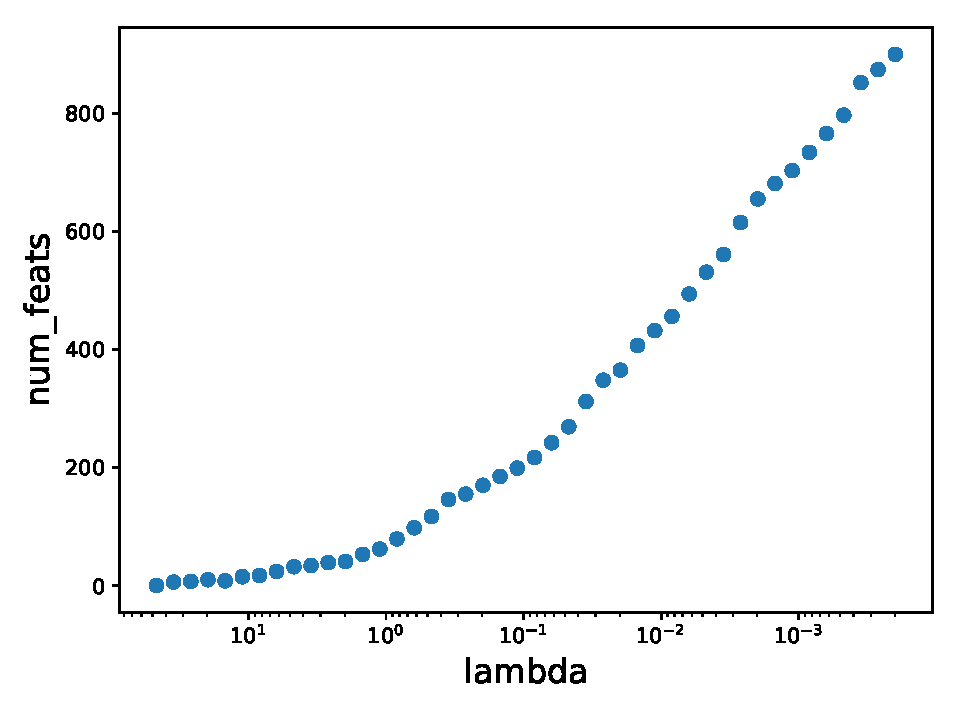
\includegraphics[width=.6\textwidth]{figures/yelp_nfeats.pdf}
				\caption{Number of nonzero features vs. $\lambda$ on Yelp data}
				\label{fig:yelp_feats}
			\end{figure}
		
		\item When trained at $\lambda=1.11$, our predictor achieves mean-squared error of 0.428 for the training set, 0.392 for the validation set, and 0.465 for the test set.




		\item The features with the largest weights are shown in Table~\ref{tab:topfeats}. These results are roughly sensible: longer reviews of better-rated restaurants from overall more-upvoted users tend to perform better. Interestingly, every feature containing \texttt{UserNumReviews} has a negative weight, suggesting that perhaps users with many reviews post a torrent of low-quality content, while users with fewer reviews have put more thought into their work.

		\begin{table}[H]
			\centering
			\begin{tabular}{c|c}
				Feature name & Weight\\\hline
				log(ReviewNumCharacters*UserUsefulVotes) &  18.915628\\
				sqrt(UserCoolVotes*BusinessNumStars)     &  18.803663\\
				log(UserNumReviews)                      & -18.129188\\
				sqrt(ReviewNumCharacters*UserCoolVotes)  &  10.729772\\
				sq(UserNumReviews*BusinessIsOpen)        & -5.546979 \\
				log(UserUsefulVotes)                     &  5.355956 \\
				log(ReviewNumLineBreaks*UserCoolVotes)   &  3.942156 \\
				log(UserCoolVotes*BusinessIsOpen)        &  3.710749 \\
				sq(ReviewNumWords*UserNumReviews)        & -3.151529 \\
				log(UserNumReviews*BusinessNumCheckins)  & -2.923991 \\
			\end{tabular}
			\caption{Top 10 highest-weighted features at optimal $\lambda$}
			\label{tab:topfeats}
		\end{table}
	\end{enumerate}














	\item We lastly consider binary classification between 2s and 7s in the MNIST set via regularized logistic regression. We choose a balanced target set $Y \in \{-1,1\}$, where $Y=-1$ for 2s and $Y = 1$ for 7s, so that our data are $\{(x_i,y_i)\}_{i=1}^n \subset \mathbb{R}^d \times \mathbb{Z}_2$. The $L_2$-regularized negative log likelihood objective to be minimized is
	%
	\begin{align*}
		J(w,b) &= \frac{1}{n} \sum_{i=1}^n \log\left[1 + \exp\left(-y_i(b+x_i^T w)\right)\right] + \lambda \|w\|_2^2.
	\end{align*}
	%
	For convenience, we define the functions
	%
	\begin{align*}
		\mu_i(w,b) &= \frac{1}{1+\exp\left[-y_i(b+x_i^T w)\right]}.
	\end{align*}.
	%
	\begin{enumerate}
		\item To do gradient descent, we need to know some gradients. First,
		\begin{align*}
			\nabla_w J(w,b) &= \frac{1}{n} \sum_{i=1}^n \frac{-y_i x_i \exp\left[-y_i(b + x_i^T w)\right]}{1 + \exp\left[-y_i(b+x_i^T w)\right]} + 2\lambda w\\
			\nabla_w J(w,b) &= -\frac{1}{n} \sum_{i=1}^n \mu_i \left(\frac{1}{\mu_i} - 1\right) y_i x_i + 2\lambda w\\
			\nabla_w J(w,b) &= \frac{1}{n} \sum_{i=1}^n (\mu_i - 1) y_i x_i + 2\lambda w.
		\end{align*}
		%
		Next,
		%
		\begin{align*}
			\nabla_b J(w,b) &= -\frac{1}{n} \sum_{i=1}^n \frac{y_i \exp\left[-y_i(b + x_i^T w)\right]}{1+\exp\left[-y_i(b+x_i^T w)\right]}\\
			\nabla_b J(w,b) &= \frac{1}{n} \sum_{i=1}^n (\mu_i -1) y_i.
		\end{align*}
		%
		We'll also want some Hessians, for Newton's method.
		%
		\begin{align*}
			\nabla^2_w J(w,b) &= \frac{1}{n} \sum_{i=1}^n y_i (\nabla_w \mu_i) x_i^T + 2\lambda I_d\\
			\nabla_w \mu_i &= \frac{y_i x_i \exp\left[-y_i(b+x_i^T w)\right]}{\left(1+\exp\left[-y_i(b+x_i^T w)\right]\right)^2} = \mu_i^2 \left(\frac{1}{\mu_i} - 1\right) y_i x_i = \mu_i (1- \mu_i) y_i x_i\\
			%
			\nabla^2_w J(w,b) &= \frac{1}{n} \sum_{i=1}^n \mu_i (1-\mu_i) y_i^2 x_i x_i^T + 2 \lambda I_d
		\end{align*}
		%
		Lastly,
		%
		\begin{align*}
			\nabla^2_b J(w,b) &= \frac{1}{n} \sum_{i=1}^n (\nabla_b \mu_i) y_i\\
			\nabla_b \mu_i &= \frac{y_i \exp\left[-y_i(b+x_i^T w)\right]}{\left(1+\exp\left[-y_i(b+x_i^T w)\right]\right)^2} = \mu_i(1-\mu_i)y_i\\
			\nabla^2_b J(w,b) &= \frac{1}{n} \sum_{i=1}^n \mu_i(1-\mu_i) y_i^2.
		\end{align*}

















		\item We implemented gradient descent on this MNIST classification problem from an initial guess of all zeros, and settled on a step size of $\eta = 0.4$ as giving reliably quick convergence and minimal overshooting issues.

		\begin{figure}[H]
			\centering
			\begin{subfigure}[t]{.45\textwidth}
				\centering
				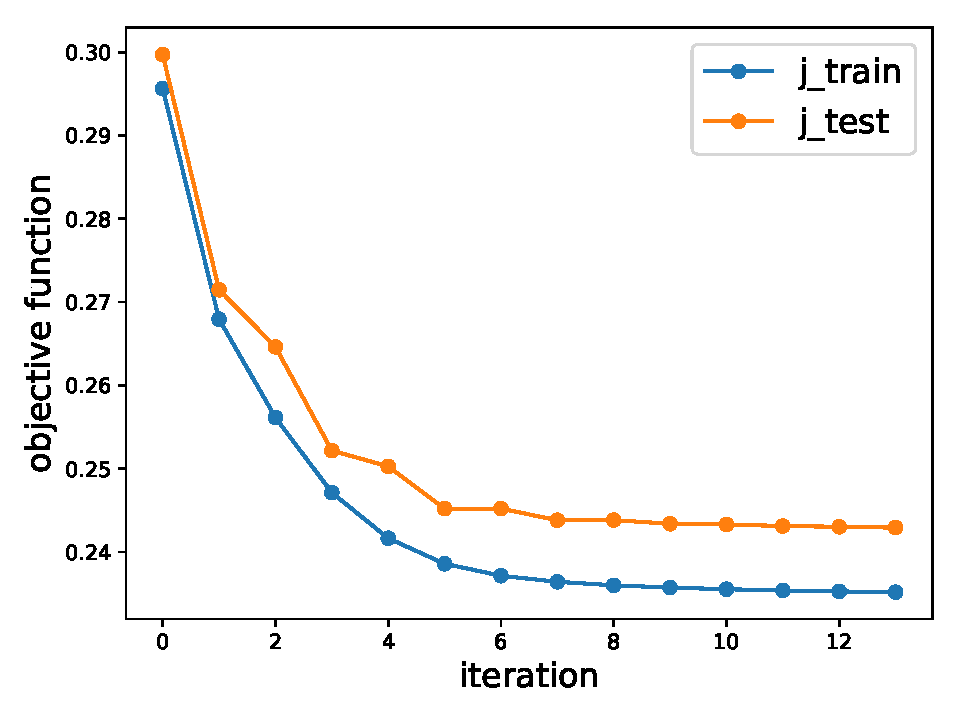
\includegraphics[width=\textwidth]{figures/mnist_gd_obj.pdf}
			\end{subfigure}
			%
			\begin{subfigure}[t]{.45\textwidth}
				\centering
				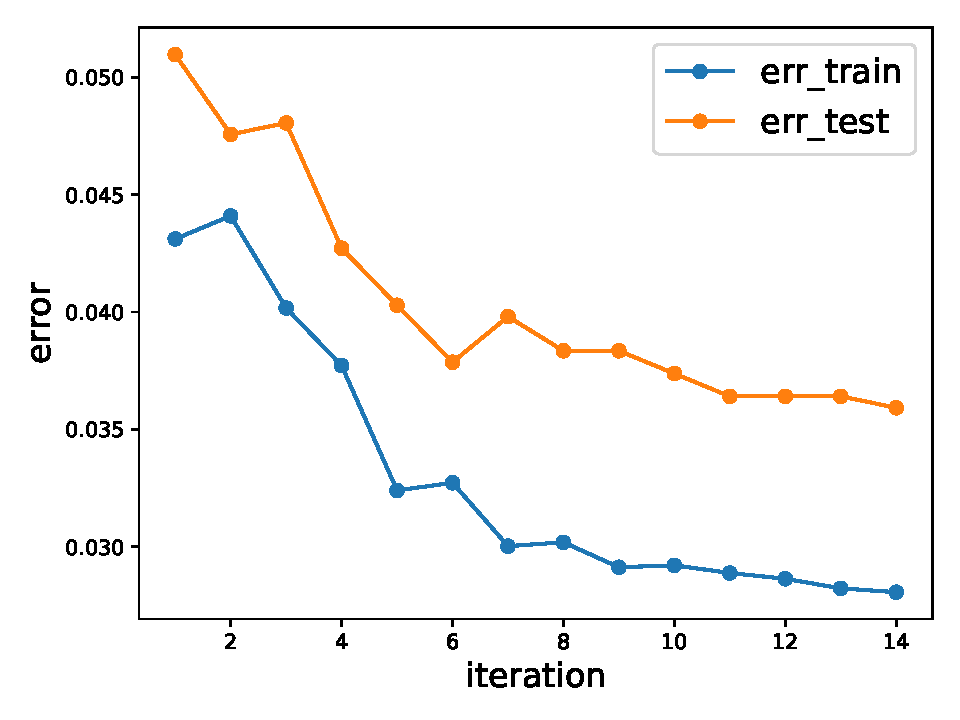
\includegraphics[width=\textwidth]{figures/mnist_gd_err.pdf}
			\end{subfigure}
			\caption{Objective and classification error at each gradient descent iteration}
		\end{figure}




		\item Stochastic gradient descent with a batch size of 1 shows a much less stable descent pattern, often showing large fluctuations in classification error as steps stumble toward the minimum.

		\begin{figure}[H]
			\centering
			\begin{subfigure}[t]{.45\textwidth}
				\centering
				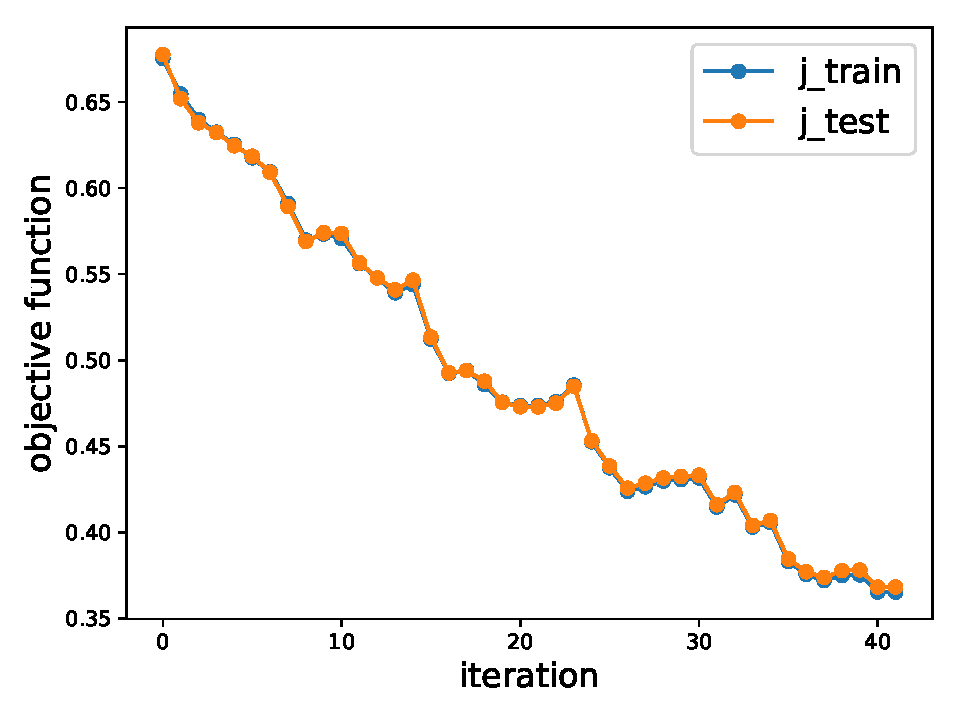
\includegraphics[width=\textwidth]{figures/mnist_sgd_1_obj.pdf}
			\end{subfigure}
			%
			\begin{subfigure}[t]{.45\textwidth}
				\centering
				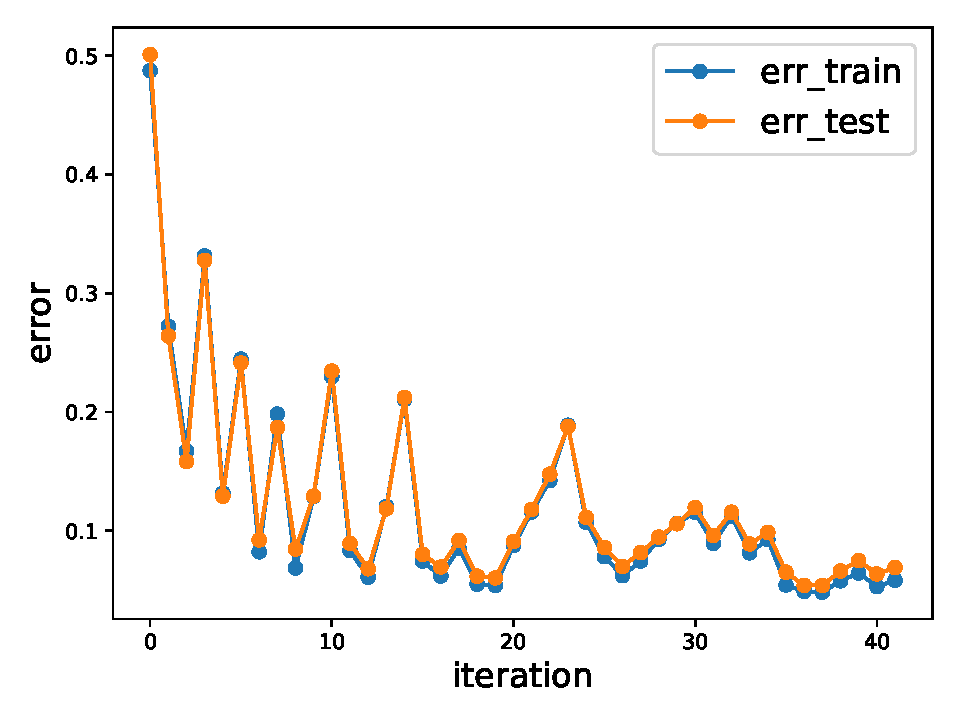
\includegraphics[width=\textwidth]{figures/mnist_sgd_1_err.pdf}
			\end{subfigure}
			\caption{Objective and classification error at each stochastic gradient descent iteration; batch size 1}
		\end{figure}

		\item Increasing batch size to 100 seems to give much more reliable steps after a relatively large first step error.


		\begin{figure}[H]
			\centering
			\begin{subfigure}{.45\textwidth}
				\centering
				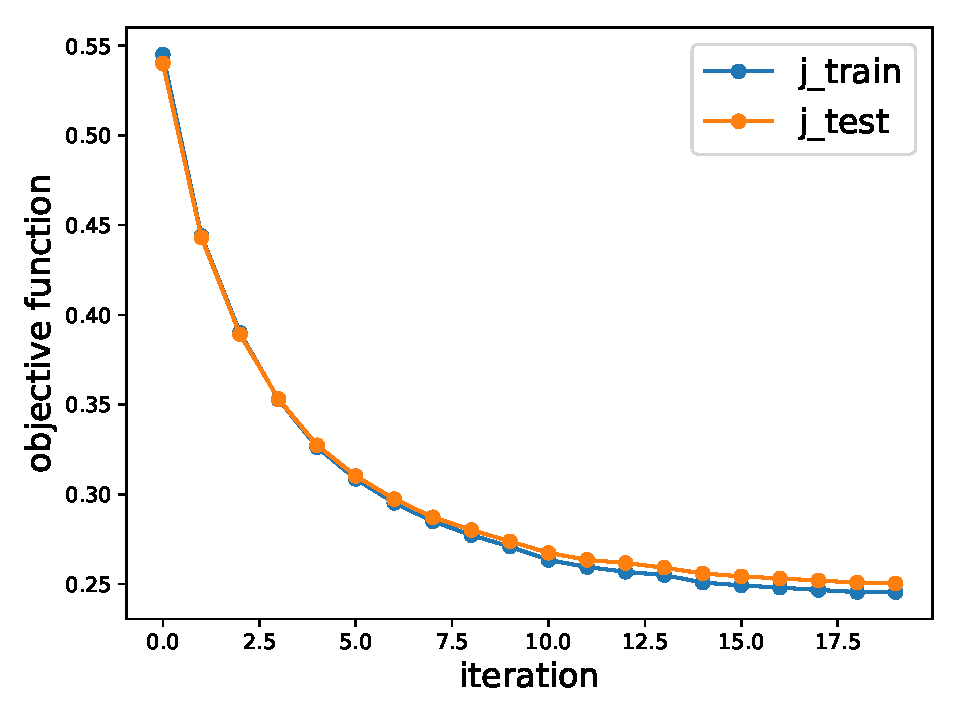
\includegraphics[width=\textwidth]{figures/mnist_sgd_100_obj.pdf}
			\end{subfigure}
			%
			\begin{subfigure}{.45\textwidth}
				\centering
				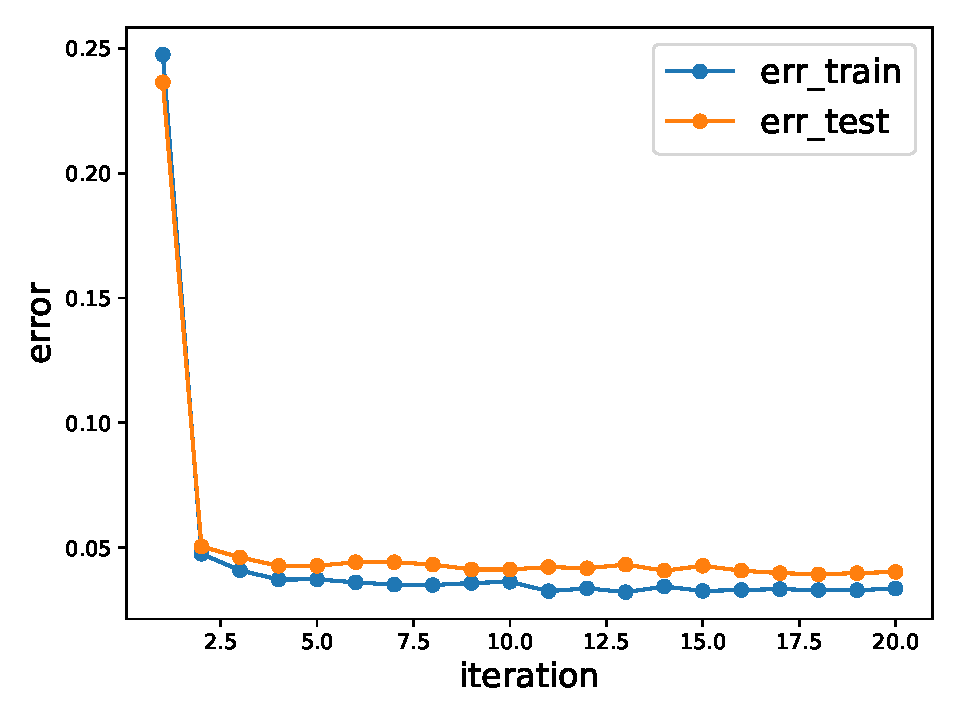
\includegraphics[width=\textwidth]{figures/mnist_sgd_100_err.pdf}
			\end{subfigure}
			\caption{Objective and classification error at each stochastic gradient descent iteration; batch size 100}
		\end{figure}

		\item We also implemented Newton's method on the same data. Although it technically took the fewest steps for the same step-size and tolerance, each individual step was much, much slower owing to the need to calculate the relatively slow Hessian for every point and then solve for the step vector. The error graph looks suspicious, but the initial error is already at least as good as any achieved with gradient descent, so I think the apparent increase is just small oscillation around an already good first iterate.


		\begin{figure}[H]
			\centering
			\begin{subfigure}{.45\textwidth}
				\centering
				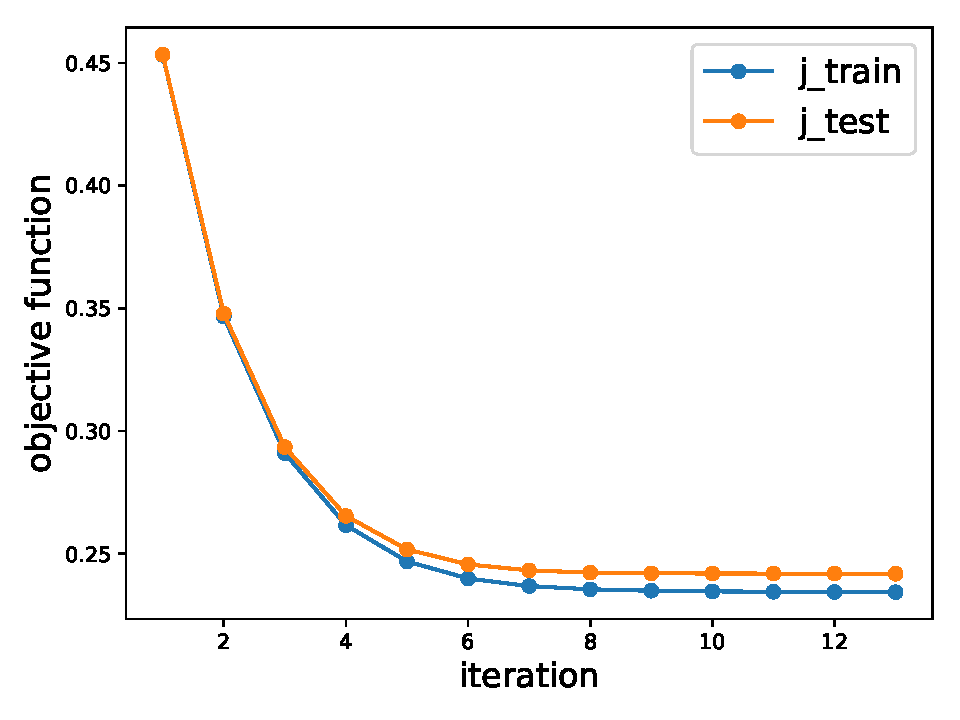
\includegraphics[width=\textwidth]{figures/mnist_newt_obj.pdf}
			\end{subfigure}
			%
			\begin{subfigure}{.45\textwidth}
				\centering
				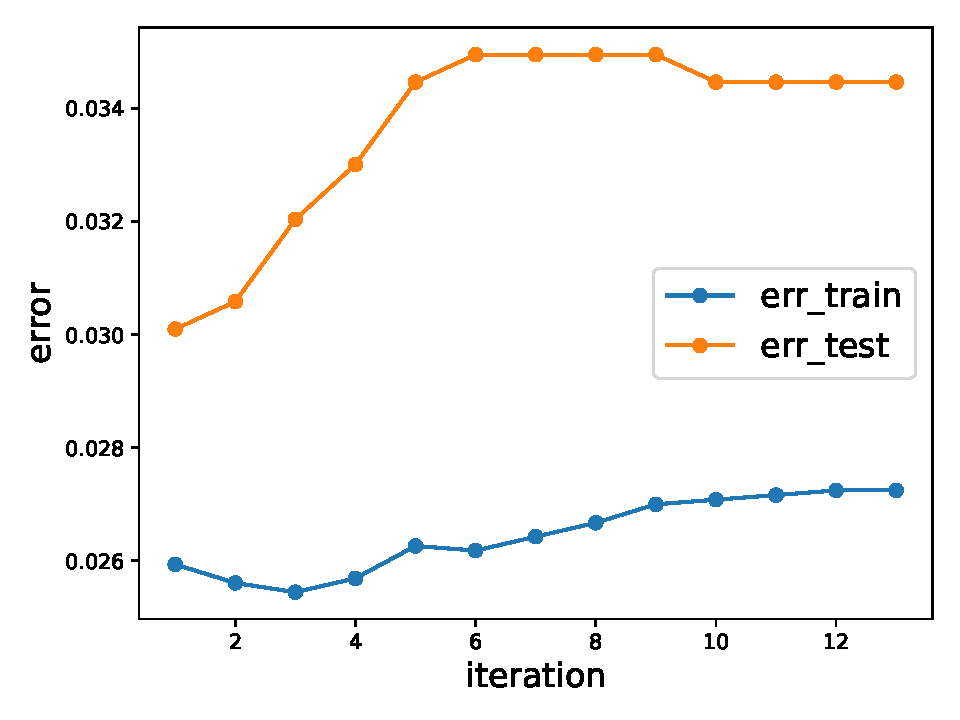
\includegraphics[width=\textwidth]{figures/mnist_newt_err.pdf}
			\end{subfigure}
			\caption{Objective and classification error at iteration of Newton's method}
		\end{figure}
	\end{enumerate}
\end{enumerate}















\clearpage
\lstinputlisting[language=Python]{code/lasso.py}
\clearpage
\lstinputlisting[language=Python]{code/synth_lasso.py}
\clearpage
\lstinputlisting[language=Python]{code/yelp_lasso.py}
\clearpage
\lstinputlisting[language=Python]{code/yelp_test.py}
\clearpage
\lstinputlisting[language=Python]{code/grad_descend.py}
\clearpage
\lstinputlisting[language=Python]{code/plotter.py}



\end{document}
